\documentclass[a4paper,12pt]{article}

\usepackage{graphicx}
\usepackage{hyperref}
\usepackage{fancyhdr}
\usepackage{titlesec}
\usepackage{geometry}
\usepackage{longtable}
\usepackage{listings}
\usepackage{xcolor}
\usepackage{float}

\geometry{margin=1in}

\titleformat{\section}{\large\bfseries}{\thesection}{1em}{}
\titleformat{\subsection}{\normalsize\bfseries}{\thesubsection}{1em}{}

\hypersetup{
    colorlinks=true,
    linkcolor=blue,
    filecolor=magenta,
    urlcolor=cyan,
}

\pagestyle{fancy}
\fancyhf{}
\rfoot{\thepage}

\lstdefinestyle{sqlstyle}{
    language=SQL,
    basicstyle=\ttfamily\footnotesize,
    keywordstyle=\color{blue}\bfseries,
    stringstyle=\color{red},
    commentstyle=\color{green!60!black},
    breaklines=true,
    frame=single,
    backgroundcolor=\color{gray!10},
    numbers=left,
    numberstyle=\tiny\color{gray},
    showstringspaces=false
}

\title{Project Report: Fraud Detection in Banking Transactions \\ \large Fundamentals of Database Systems (CSE462a)}
\author{
Youssef Basem (240919), Moaaz Tamer (245789), \\ Ramy Emad (ID\_TBD) \\
\texttt{Youssef.bassem1@msa.edu.eg, moaaz.tamer@msa.edu.eg} \\
\texttt{ramy.emad@msa.edu.eg} \\
Supervised by: Dr. Ahmed Ayoub}
\date{\today}

\begin{document}

\maketitle

\begin{abstract}
This document presents a detailed report on the project titled \textbf{Fraud Detection in Banking Transactions}. The system is designed to monitor and detect fraudulent activities in banking through transaction tracking, anomaly detection, flagged accounts, and fraud reports. The report covers the problem statement, objectives, database design (ERD and normalization), implementation details including stored procedures, triggers, and transactions, query optimization with indexing and execution plan analysis, data integrity and security measures, and conclusions. The database is implemented in MySQL 8.0 with 11 normalized tables, 20+ records per table, and comprehensive fraud detection logic.
\end{abstract}
\newpage

\tableofcontents
\clearpage
\newpage

%==============================================================
\section{Introduction}
%==============================================================

\subsection{Problem Statement}
Financial fraud is a growing concern in the banking industry, costing billions of dollars annually. Traditional manual monitoring is insufficient to handle the volume and velocity of modern banking transactions. Banks need automated systems that can track transactions in real-time, detect anomalous patterns, flag suspicious accounts, and generate investigation reports. This project addresses the need for a robust relational database system that serves as the backbone of a fraud detection platform, enabling analysts to identify, investigate, and resolve fraudulent activities efficiently.

\subsection{Objectives}
\begin{itemize}
    \item Design a normalized relational database schema (3NF) for fraud detection in banking.
    \item Implement transaction tracking with comprehensive metadata (channel, IP, device, location).
    \item Create configurable fraud detection rules for various anomaly patterns.
    \item Build stored procedures for automated fraud scanning (high-value, velocity, geographic anomalies).
    \item Implement triggers for real-time audit logging and alert generation.
    \item Optimize query performance through strategic indexing for large datasets.
    \item Enforce data integrity through constraints and role-based access control.
    \item Generate fraud investigation reports and risk scoring for customers.
\end{itemize}

\subsection{Scope}
The system covers the following functional areas:
\begin{itemize}
    \item \textbf{Core Banking}: Customer profiles, bank accounts, branch management.
    \item \textbf{Transaction Monitoring}: Full transaction lifecycle with metadata capture.
    \item \textbf{Fraud Detection}: Configurable rules, automated alert generation, severity classification.
    \item \textbf{Investigation}: Fraud reports, account flagging, risk scoring.
    \item \textbf{Security}: User roles, audit logging, login attempt tracking.
\end{itemize}
\textbf{Limitations}: The system focuses on the database layer; front-end applications and real-time streaming are out of scope. Machine learning-based detection is represented through configurable rule thresholds rather than actual ML models.

%==============================================================
\section{Database Design}
%==============================================================

\subsection{Entity-Relationship Diagram (ERD)}
The ERD below illustrates the complete database design using Chen's notation (rectangles for entities, diamonds for relationships, ovals for attributes, with cardinality labels). The system consists of 11 entities organized into three logical layers: Core Banking (Branches, Customers, Accounts), Transaction Processing (Transactions), and Fraud Detection (FraudAlerts, FraudRules, FlaggedAccounts, FraudReports, Users, AuditLog, LoginAttempts).

\begin{figure}[H]
    \centering
    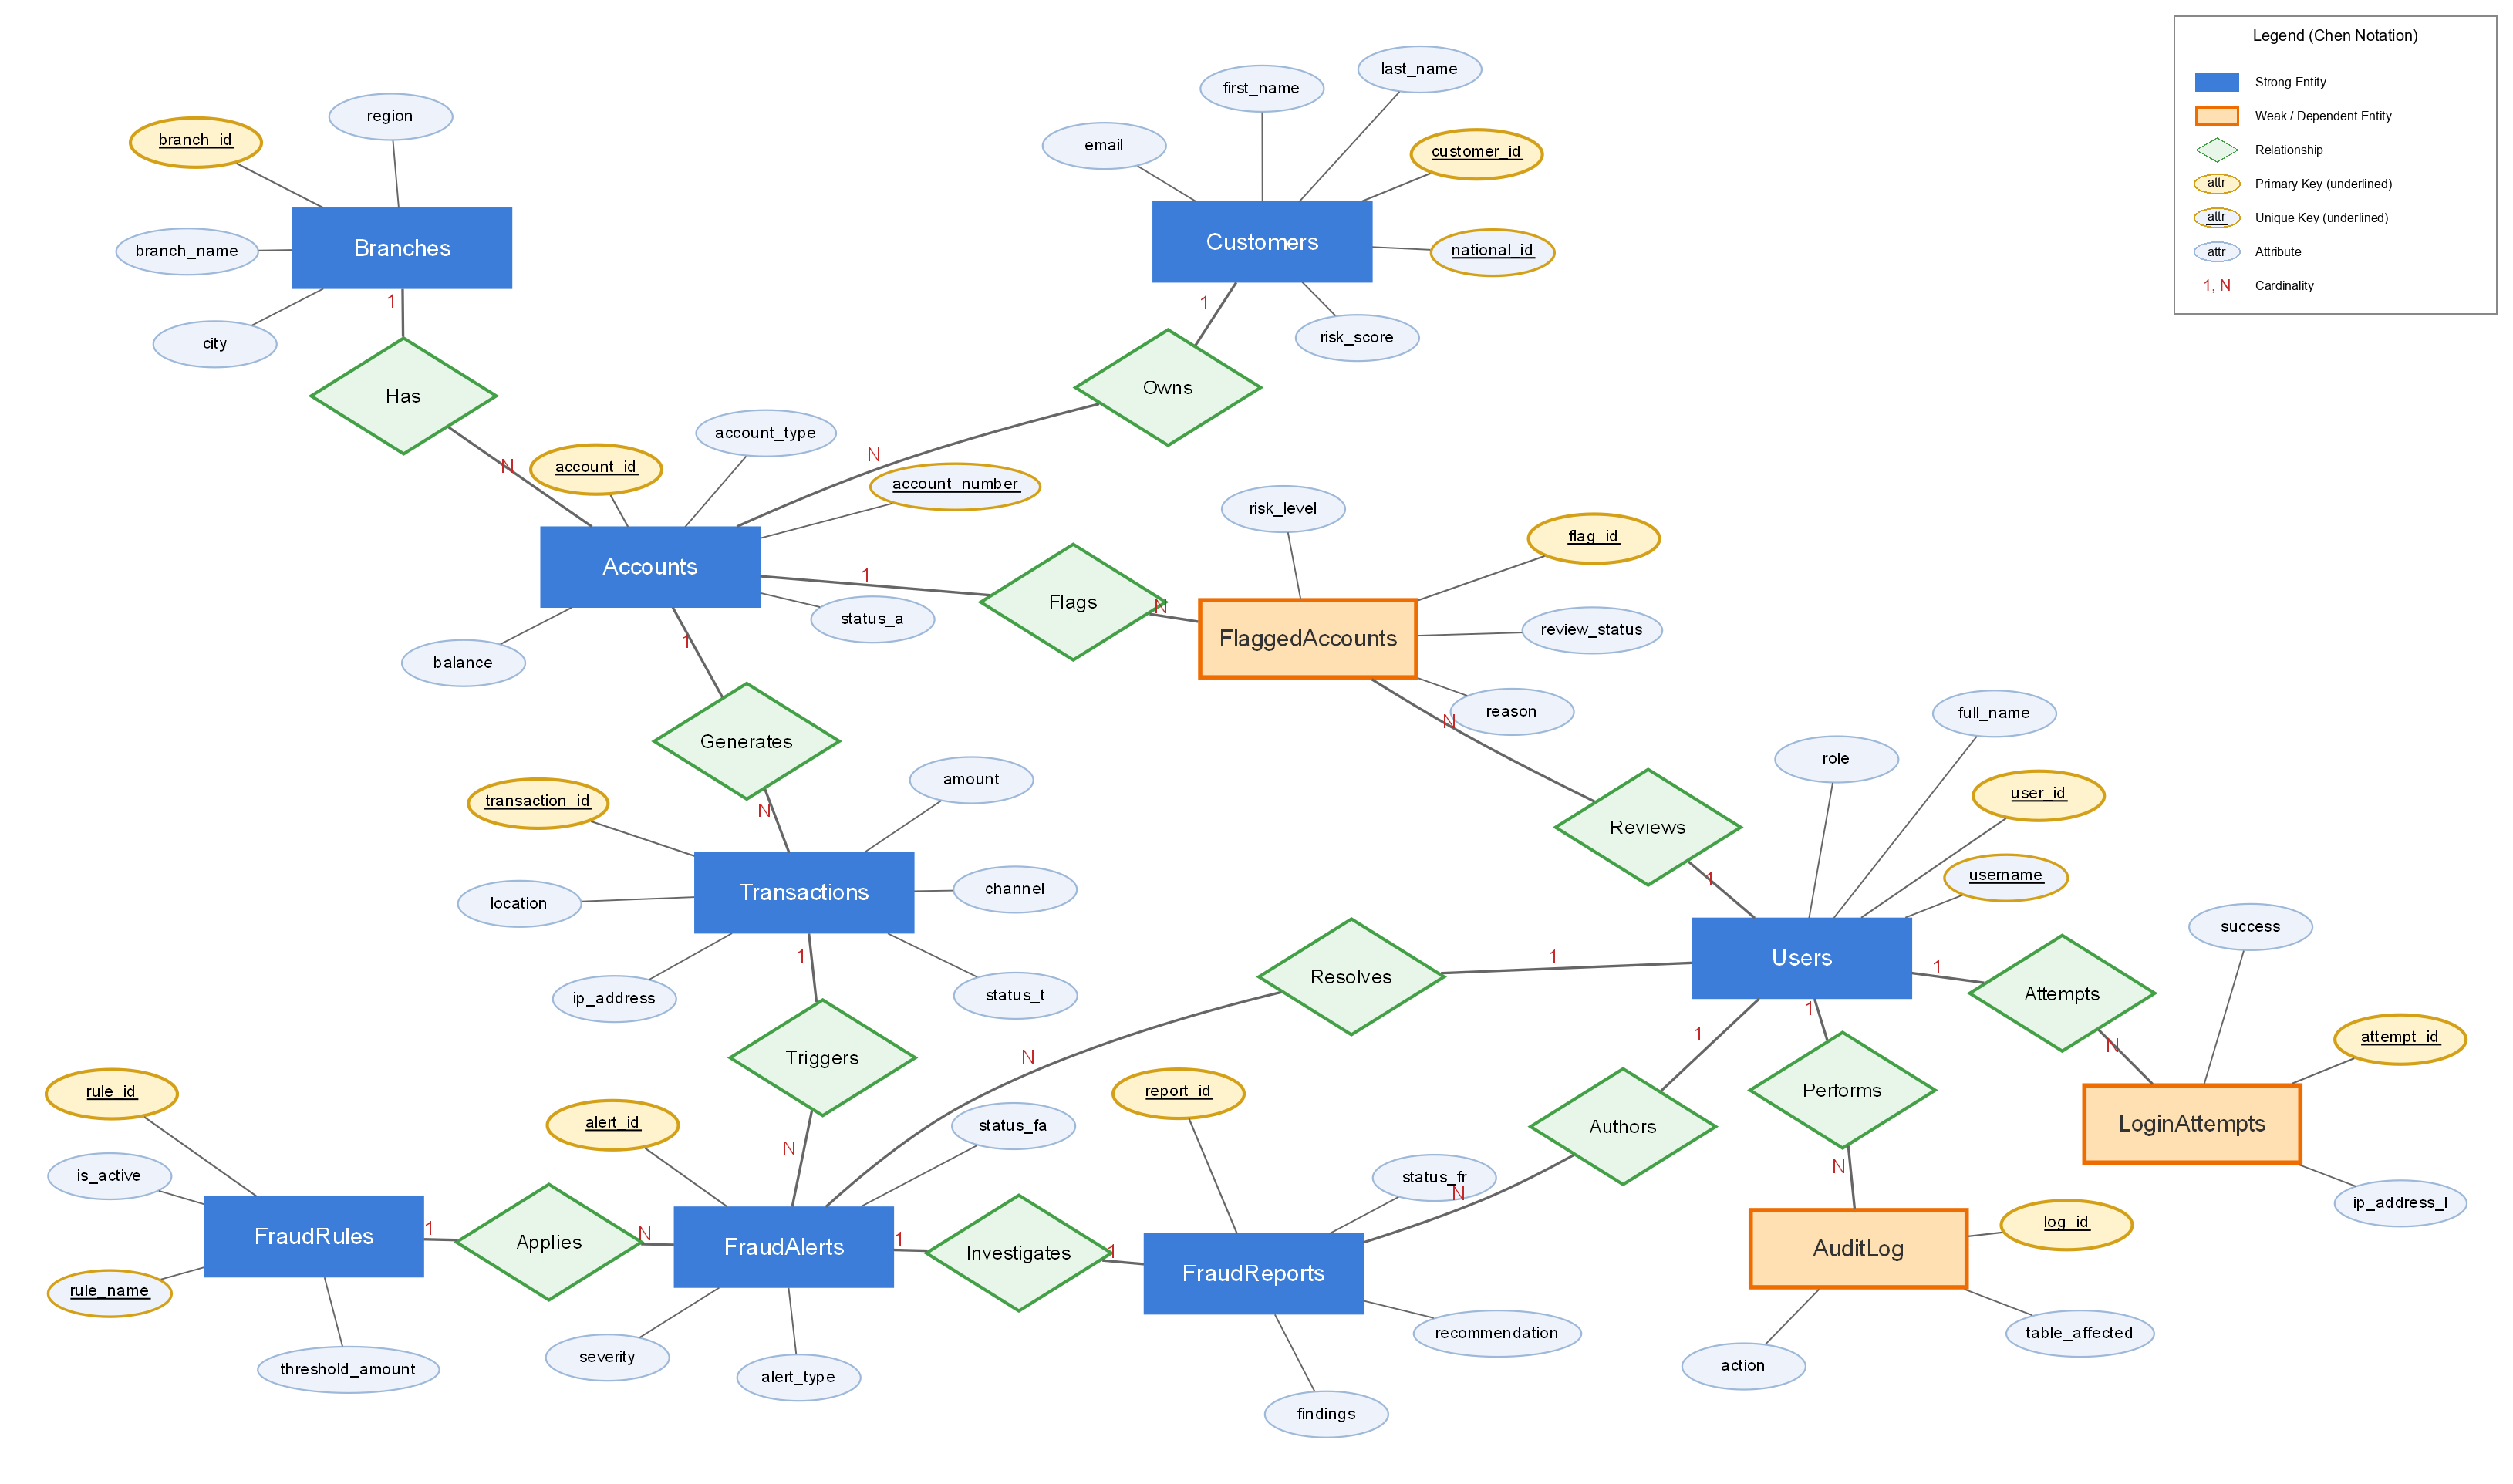
\includegraphics[width=\textwidth]{chen_erd.png}
    \caption{Entity-Relationship Diagram --- Chen's Notation}
    \label{fig:erd_chen}
\end{figure}

Figure~\ref{fig:erd_crows} presents the same schema using Crow's Foot notation, which provides a more detailed physical view including data types, nullability constraints, and foreign key references for each table.

\begin{figure}[H]
    \centering
    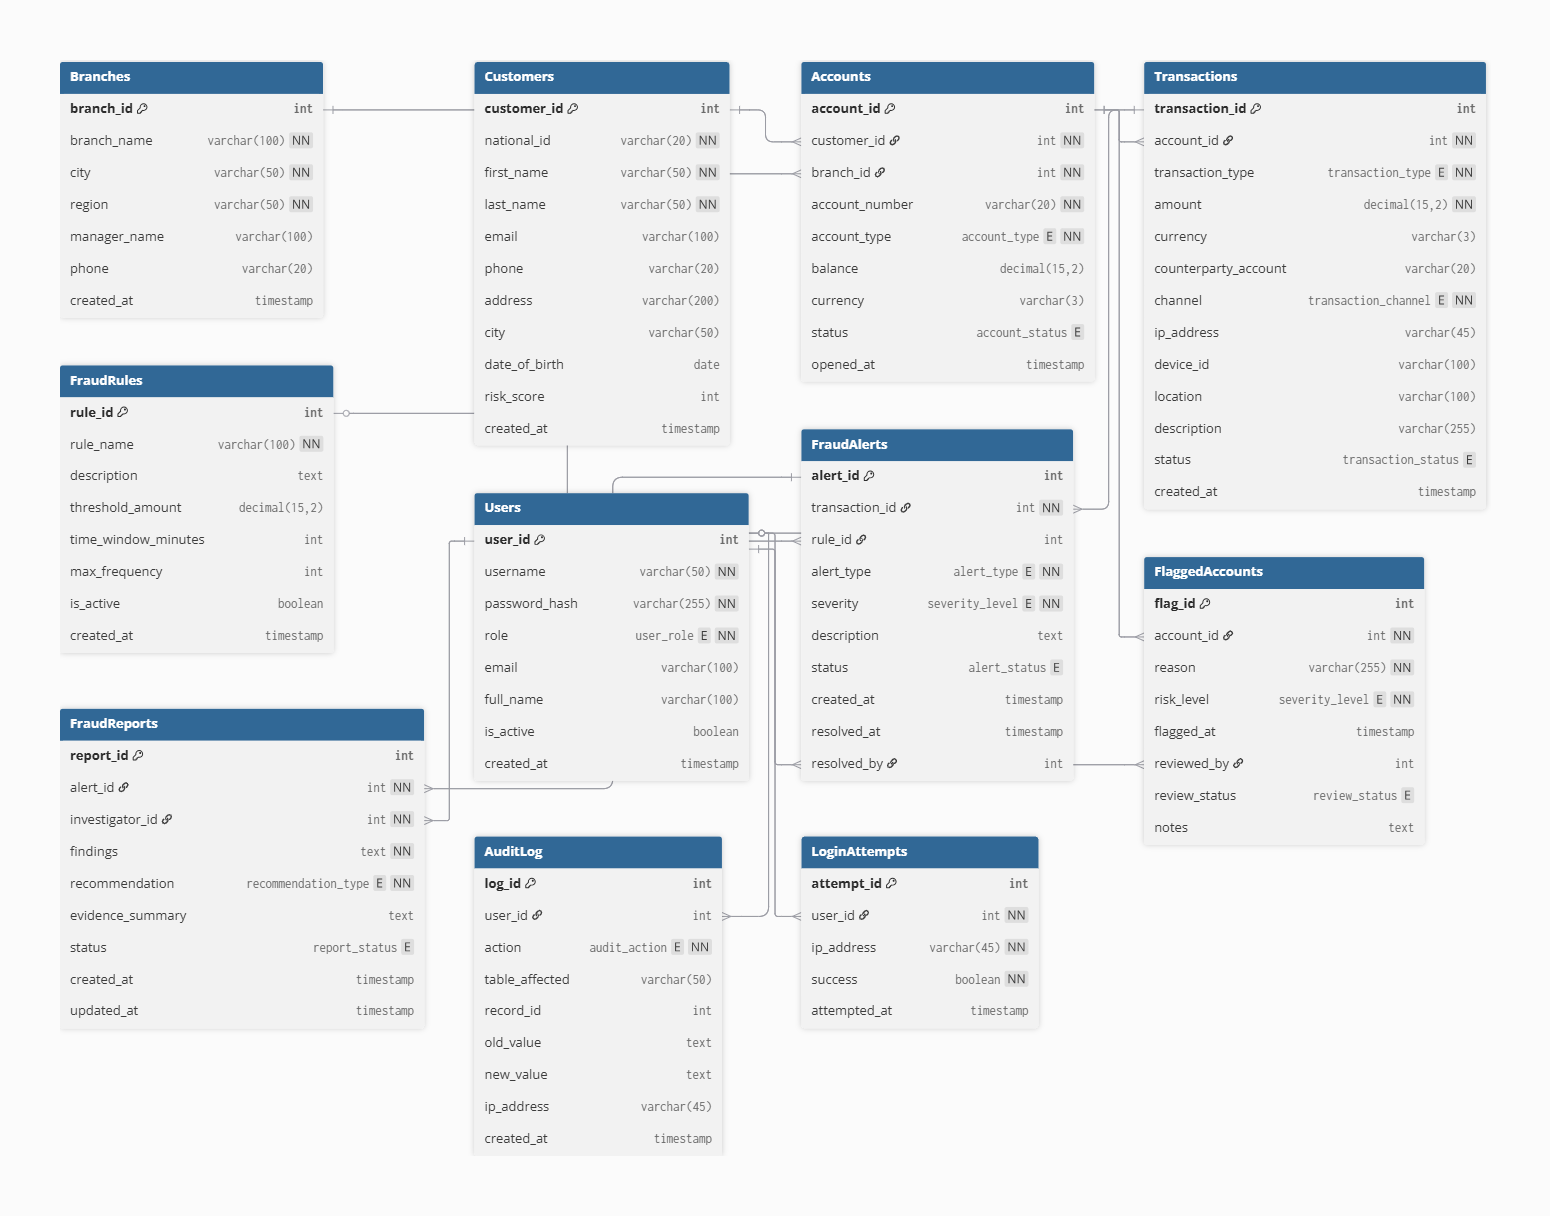
\includegraphics[width=\textwidth]{crows_foot.png}
    \caption{Entity-Relationship Diagram --- Crow's Foot Notation}
    \label{fig:erd_crows}
\end{figure}

\textbf{Key Relationships:}
\begin{itemize}
    \item Branches (1) $\rightarrow$ (N) Accounts: Each branch hosts multiple accounts.
    \item Customers (1) $\rightarrow$ (N) Accounts: A customer can have multiple accounts.
    \item Accounts (1) $\rightarrow$ (N) Transactions: Each account has many transactions.
    \item Transactions (1) $\rightarrow$ (N) FraudAlerts: A transaction can trigger multiple alerts.
    \item FraudRules (1) $\rightarrow$ (N) FraudAlerts: Rules generate alerts.
    \item FraudAlerts (1) $\rightarrow$ (1) FraudReports: Each alert may have one investigation report.
    \item Users resolve alerts, review flagged accounts, and author reports.
\end{itemize}

\subsection{Normalization}
The database is designed in \textbf{Third Normal Form (3NF)}:

\textbf{1NF}: All tables have atomic values. No repeating groups. Each column contains a single value (e.g., customer name is split into first\_name and last\_name).

\textbf{2NF}: All non-key attributes are fully functionally dependent on the entire primary key. Since all tables use single-column surrogate primary keys (AUTO\_INCREMENT), partial dependencies are eliminated by design.

\textbf{3NF}: No transitive dependencies exist.
\begin{itemize}
    \item Branch information is separated from Accounts (branch\_id FK instead of embedding branch details).
    \item Customer data is separated from Accounts.
    \item Fraud rules are in a separate table referenced by FraudAlerts via rule\_id FK.
    \item User information (investigators, reviewers) is referenced via FK rather than stored inline.
\end{itemize}

No denormalization was applied as the schema is efficient for the expected query patterns. Views are used to provide denormalized read access without compromising the normalized base tables.

\subsection{Schema Design}
The complete relational schema (detailed in Figure~\ref{fig:erd_crows}) consists of 11 tables with the following key design decisions:
\begin{itemize}
    \item \textbf{ENUM types} for status fields (account status, alert severity, transaction type) to enforce domain constraints at the database level.
    \item \textbf{Surrogate keys} (AUTO\_INCREMENT) for all primary keys for consistent referencing.
    \item \textbf{Composite indexes} on frequently queried column combinations.
    \item \textbf{CHECK constraints} on risk\_score (0--100) and amount ($> 0$).
    \item \textbf{SHA2 hashing} for password storage in the Users table.
\end{itemize}

\newpage

%==============================================================
\section{Implementation}
%==============================================================

\subsection{Database Tables}
The system comprises 11 tables:

\begin{longtable}{|p{3.5cm}|p{4cm}|p{6cm}|}
\hline
\textbf{Table} & \textbf{Key Columns} & \textbf{Purpose} \\
\hline
Branches & branch\_id (PK), branch\_name, city, region & Bank branch locations \\
\hline
Customers & customer\_id (PK), national\_id (UK), risk\_score & Customer profiles with fraud risk scores \\
\hline
Accounts & account\_id (PK), customer\_id (FK), branch\_id (FK), status & Bank accounts linked to customers and branches \\
\hline
Transactions & transaction\_id (PK), account\_id (FK), amount, channel, ip\_address, location & Complete transaction records with metadata \\
\hline
FraudRules & rule\_id (PK), rule\_name (UK), threshold\_amount, time\_window & Configurable fraud detection rules \\
\hline
FraudAlerts & alert\_id (PK), transaction\_id (FK), rule\_id (FK), severity, status & Alerts generated by fraud detection \\
\hline
FlaggedAccounts & flag\_id (PK), account\_id (FK), risk\_level, review\_status & Accounts under investigation \\
\hline
FraudReports & report\_id (PK), alert\_id (FK), investigator\_id (FK), recommendation & Investigation reports \\
\hline
Users & user\_id (PK), username (UK), password\_hash, role & System users (Admin, Analyst, Teller, Auditor) \\
\hline
AuditLog & log\_id (PK), user\_id (FK), action, table\_affected & System audit trail \\
\hline
LoginAttempts & attempt\_id (PK), user\_id (FK), ip\_address, success & Login tracking for security \\
\hline
\end{longtable}

Each table contains at least 20 sample records with realistic banking data, including intentionally fraudulent patterns such as:
\begin{itemize}
    \item Rapid successive transfers (3 transfers within 10 minutes)
    \item Large international wires during midnight hours (1--5 AM)
    \item Geographic impossibilities (Dubai to Nairobi in 45 minutes)
    \item Potential structuring (amounts near \$10,000 reporting threshold)
\end{itemize}

\subsection{SQL Queries}

\textbf{CRUD Operations:}
\begin{lstlisting}[style=sqlstyle, caption=SELECT - Active accounts with customer info]
SELECT c.first_name, c.last_name, a.account_number, 
       a.account_type, a.balance, a.status
FROM Customers c 
JOIN Accounts a ON c.customer_id = a.customer_id
WHERE a.status = 'Active' ORDER BY a.balance DESC;
\end{lstlisting}

\begin{lstlisting}[style=sqlstyle, caption=UPDATE - Resolve a fraud alert]
UPDATE FraudAlerts 
SET status = 'Resolved', resolved_at = NOW(), resolved_by = 3
WHERE alert_id = 3;
\end{lstlisting}

\textbf{JOIN Operations:}
\begin{lstlisting}[style=sqlstyle, caption=Multi-table JOIN - Full fraud investigation view]
SELECT c.first_name, c.last_name, c.risk_score,
       a.account_number, t.amount, t.channel, t.location,
       fa.alert_type, fa.severity, fa.status AS alert_status
FROM Customers c
INNER JOIN Accounts a ON c.customer_id = a.customer_id
INNER JOIN Transactions t ON a.account_id = t.account_id
INNER JOIN FraudAlerts fa ON t.transaction_id = fa.transaction_id
ORDER BY fa.severity DESC, t.amount DESC;
\end{lstlisting}

\textbf{Aggregate Functions:}
\begin{lstlisting}[style=sqlstyle, caption=Fraud amounts by alert type with aggregates]
SELECT fa.alert_type, COUNT(*) AS alert_count,
       SUM(t.amount) AS total_flagged_amount, 
       AVG(t.amount) AS avg_flagged_amount
FROM FraudAlerts fa 
JOIN Transactions t ON fa.transaction_id = t.transaction_id
GROUP BY fa.alert_type ORDER BY total_flagged_amount DESC;
\end{lstlisting}

\textbf{Subqueries:}
\begin{lstlisting}[style=sqlstyle, caption=Accounts with transactions exceeding 3x their average]
SELECT a.account_number, t.amount, t.created_at, t.channel
FROM Transactions t
JOIN Accounts a ON t.account_id = a.account_id
WHERE t.amount > 3 * (
    SELECT AVG(t2.amount) FROM Transactions t2 
    WHERE t2.account_id = t.account_id
) ORDER BY t.amount DESC;
\end{lstlisting}

\subsection{Stored Procedures, Triggers, Transactions}

\textbf{Stored Procedures (5 implemented):}

\begin{enumerate}
    \item \texttt{sp\_detect\_high\_value\_fraud(threshold)} -- Scans all transactions above a threshold amount, automatically creates fraud alerts with appropriate severity levels (Critical $\geq$ \$50k, High $\geq$ \$20k, Medium $\geq$ \$10k). Uses a cursor to iterate through unprocessed transactions.
    
    \item \texttt{sp\_detect\_velocity\_fraud(account\_id, time\_window, max\_count)} -- Detects rapid-fire transactions by counting transactions within a specified time window. Generates alerts when the count exceeds the maximum allowed frequency.
    
    \item \texttt{sp\_generate\_fraud\_report(alert\_id, investigator\_id, findings, recommendation)} -- Creates a formal investigation report linked to a fraud alert, validates the alert exists, and updates the alert status to Under\_Review.
    
    \item \texttt{sp\_update\_risk\_score(customer\_id)} -- Calculates a dynamic risk score (0--100) based on confirmed frauds ($\times$25), open alerts ($\times$10), and total flagged amount (scaled by \$10k increments).
    
    \item \texttt{sp\_fund\_transfer(from, to, amount)} -- Performs a safe fund transfer within a transaction, checking account status and balance before proceeding. Automatically flags transfers $\geq$ \$10,000.
\end{enumerate}

\begin{lstlisting}[style=sqlstyle, caption=Fund Transfer Stored Procedure (excerpt)]
CREATE PROCEDURE sp_fund_transfer(
    IN p_from INT, IN p_to INT, IN p_amount DECIMAL(15,2))
BEGIN
    DECLARE v_balance DECIMAL(15,2);
    DECLARE v_from_status VARCHAR(10);
    DECLARE EXIT HANDLER FOR SQLEXCEPTION 
        BEGIN ROLLBACK; RESIGNAL; END;
    START TRANSACTION;
    SELECT balance, status INTO v_balance, v_from_status 
        FROM Accounts WHERE account_id = p_from FOR UPDATE;
    IF v_from_status != 'Active' THEN
        SIGNAL SQLSTATE '45000' 
        SET MESSAGE_TEXT = 'Source account is not active';
    END IF;
    IF v_balance < p_amount THEN
        SIGNAL SQLSTATE '45000' 
        SET MESSAGE_TEXT = 'Insufficient balance';
    END IF;
    UPDATE Accounts SET balance = balance - p_amount 
        WHERE account_id = p_from;
    UPDATE Accounts SET balance = balance + p_amount 
        WHERE account_id = p_to;
    COMMIT;
END
\end{lstlisting}

\textbf{Triggers (3 implemented):}
\begin{enumerate}
    \item \texttt{trg\_after\_transaction\_insert} -- Fires after each new transaction. Logs high-value transactions ($\geq$ \$10k) and midnight transactions ($\geq$ \$5k between 1--4 AM) to the AuditLog.
    \item \texttt{trg\_after\_alert\_update} -- Fires when a fraud alert status changes to a terminal state (Confirmed\_Fraud, Resolved, False\_Positive). Records the status change in AuditLog.
    \item \texttt{trg\_account\_status\_change} -- Fires when an account status changes (e.g., Active $\rightarrow$ Frozen). Logs the change for audit compliance.
\end{enumerate}

\textbf{ACID Transactions:}
\begin{enumerate}
    \item Fund transfer between accounts with balance verification and rollback on failure.
    \item Batch fraud alert status update with transactional consistency.
    \item Account freeze with cascading flagged account creation.
\end{enumerate}

%==============================================================
\section{Query Optimization}
%==============================================================

Strategic indexing was implemented to optimize the most critical query patterns:

{\small
\begin{longtable}{|p{6cm}|p{4.5cm}|p{4cm}|}
\hline
\textbf{Index} & \textbf{Target Query Pattern} & \textbf{EXPLAIN Result} \\
\hline
\texttt{idx\_transactions\_account\_date} \newline (account\_id, created\_at) & Transactions by account within date range & type=range, Using index condition \\
\hline
\texttt{idx\_transactions\_amount} \newline (amount) & High-value transaction scans & type=range, Using index condition \\
\hline
\texttt{idx\_fraud\_alerts\_status\_severity} \newline (status, severity) & Alert dashboard filtering & type=ref, key=idx (exact match) \\
\hline
\texttt{idx\_customers\_national\_id} \newline (national\_id) & Customer lookup by national ID & type=const (single row) \\
\hline
\end{longtable}
}

\textbf{EXPLAIN Analysis Results:}
\begin{itemize}
    \item \textbf{Account transaction lookup}: Uses composite index \texttt{idx\_transactions\_account\_date} with \texttt{type=range}, scanning only 1 row instead of full table scan.
    \item \textbf{High-value scan}: Uses \texttt{idx\_transactions\_amount} with \texttt{type=range}, filtering to 10 candidate rows.
    \item \textbf{Critical open alerts}: Uses \texttt{idx\_fraud\_alerts\_status\_severity} with exact ref lookup, returning 1 matching row directly.
    \item \textbf{National ID lookup}: Uses the UNIQUE constraint index with \texttt{type=const}, the fastest possible access method.
\end{itemize}

Additional optimization techniques:
\begin{itemize}
    \item \textbf{Views} (vw\_fraud\_dashboard, vw\_suspicious\_transactions, vw\_account\_risk\_profile) provide pre-computed denormalized read access without compromising base table normalization.
    \item \textbf{Covering indexes} on high-frequency query columns reduce disk I/O.
    \item \textbf{FOR UPDATE} locking in the fund transfer procedure prevents phantom reads during concurrent access.
\end{itemize}

%==============================================================
\section{Data Integrity and Security}
%==============================================================

\subsection{Constraints and Data Validation}
\begin{itemize}
    \item \textbf{Primary Keys}: All 11 tables use AUTO\_INCREMENT surrogate keys.
    \item \textbf{Foreign Keys}: 12 foreign key constraints enforce referential integrity across tables. ON DELETE CASCADE is used for Customers $\rightarrow$ Accounts.
    \item \textbf{UNIQUE Constraints}: national\_id, email (Customers), account\_number (Accounts), username (Users), rule\_name (FraudRules).
    \item \textbf{CHECK Constraints}: risk\_score BETWEEN 0 AND 100, amount $>$ 0.
    \item \textbf{ENUM Types}: Enforce valid values for status fields, transaction types, channels, account types, severity levels, and user roles.
    \item \textbf{NOT NULL}: Applied to all critical fields (names, amounts, types).
    \item \textbf{DEFAULT Values}: Timestamps default to CURRENT\_TIMESTAMP, risk\_score defaults to 0, account status defaults to 'Active'.
\end{itemize}

\subsection{Access Control and Security Measures}
\textbf{Role-Based Access Control (RBAC):}
\begin{longtable}{|l|p{8cm}|}
\hline
\textbf{Role} & \textbf{Permissions} \\
\hline
fraud\_admin & Full access to all tables and operations \\
\hline
fraud\_analyst & SELECT on all tables; INSERT/UPDATE on FraudAlerts, FraudReports, FlaggedAccounts, AuditLog \\
\hline
bank\_teller & SELECT only on Transactions, Customers, Accounts \\
\hline
\end{longtable}

\textbf{Security Measures:}
\begin{itemize}
    \item \textbf{Password Hashing}: User passwords stored using SHA2-256 hashing.
    \item \textbf{Login Monitoring}: LoginAttempts table tracks all login attempts with IP addresses. Multiple failed attempts (e.g., 5 failures in 5 minutes) trigger security alerts.
    \item \textbf{Audit Trail}: AuditLog captures all data modifications with before/after values, user ID, and timestamp for forensic analysis.
    \item \textbf{Parameterized Procedures}: Stored procedures use parameterized inputs, preventing SQL injection attacks.
\end{itemize}

%==============================================================
\section{Results and Discussion}
%==============================================================

\subsection{Testing and Validation}
The system was validated through the following tests:
\begin{itemize}
    \item \textbf{Data Integrity}: All 11 tables successfully created with 20+ records each. Foreign key constraints verified through cascading operations.
    \item \textbf{Query Correctness}: All SELECT, JOIN, aggregate, and subquery operations return expected results. The fraud dashboard view correctly reports 3 open alerts, 9 under review, 5 confirmed frauds, and \$216,000 in confirmed fraud amount.
    \item \textbf{Stored Procedures}: All 5 procedures tested successfully---fund transfers correctly debit/credit accounts, fraud detection scans identify suspicious transactions, risk scoring produces meaningful scores.
    \item \textbf{Triggers}: All 3 triggers verified---AuditLog entries automatically created on transaction inserts and status changes.
    \item \textbf{Index Performance}: EXPLAIN analysis confirms all strategic indexes are utilized by the query optimizer, eliminating full table scans.
    \item \textbf{ACID Compliance}: Fund transfer transactions correctly rollback on insufficient balance, maintaining data consistency.
\end{itemize}

\subsection{Challenges and Limitations}
\begin{itemize}
    \item \textbf{Real-time Processing}: The current design uses batch-oriented stored procedures rather than real-time event streaming, which would be needed for production deployment.
    \item \textbf{Rule Complexity}: The fraud rules table supports threshold-based detection but lacks support for complex pattern matching (e.g., graph-based fraud networks).
    \item \textbf{Scalability}: For production datasets with millions of transactions, additional partitioning strategies and materialized views would be necessary.
    \item \textbf{Machine Learning Integration}: The risk scoring is formula-based; integrating ML models would require an external scoring service and API layer.
\end{itemize}

\newpage
%==============================================================
\section{Conclusion}
%==============================================================

This project successfully demonstrates a comprehensive fraud detection database system for banking transactions. The system implements 11 normalized tables in 3NF, 5 stored procedures for automated fraud detection and investigation workflows, 3 triggers for audit compliance, strategic indexing that eliminates full table scans, and role-based access control for security.

Key achievements include:
\begin{itemize}
    \item A configurable rule-based fraud detection engine
    \item Dynamic customer risk scoring based on fraud history
    \item Complete audit trail for regulatory compliance
    \item Query optimization with verified EXPLAIN execution plans
\end{itemize}

Future improvements could include:
\begin{itemize}
    \item Integration with machine learning models for predictive fraud detection
    \item Real-time transaction streaming using MySQL event scheduling
    \item Geographic visualization of fraud patterns
    \item API layer for integration with banking front-end applications
\end{itemize}

%==============================================================
\section{References}
%==============================================================

\begin{enumerate}
    \item R. Elmasri and S. Navathe, \textit{Fundamentals of Database Systems}, 7th ed. Pearson, 2016.
    \item A. Silberschatz, H. F. Korth, and S. Sudarshan, \textit{Database System Concepts}, 7th ed. McGraw-Hill, 2019.
    \item MySQL 8.0 Reference Manual, Oracle Corporation, 2024. [Online]. Available: \url{https://dev.mysql.com/doc/refman/8.0/en/}
    \item S. Panigrahi, A. Kundu, S. Sural, and A. K. Majumdar, ``Credit card fraud detection: A fusion approach using Dempster-Shafer theory and Bayesian learning,'' \textit{Information Fusion}, vol. 10, no. 4, pp. 354--363, 2009.
    \item R. J. Bolton and D. J. Hand, ``Statistical fraud detection: A review,'' \textit{Statistical Science}, vol. 17, no. 3, pp. 235--255, 2002.
\end{enumerate}

\end{document}
